\documentclass[11pt, a4paper]{article}

% --- Packages ---
\usepackage[utf8]{inputenc}
\usepackage[margin=1in]{geometry}
\usepackage{amsmath, amssymb, amsthm}
\usepackage{graphicx}
\usepackage{booktabs}
\usepackage{float}
\usepackage{hyperref}
\usepackage{emptypage}

\usepackage{xcolor}
\usepackage{tikz}
\usetikzlibrary{shapes.geometric, arrows.meta, positioning, fit, backgrounds}
\usepackage{cite}
\usepackage{titlesec}
\usepackage{caption}
\usepackage{subcaption}
\usepackage{authblk}

% --- Custom Colors (From your earlier preamble) ---
\definecolor{myNavy}{RGB}{0, 30, 90}
\definecolor{codeComment}{RGB}{34, 139, 34}
\definecolor{myRed}{RGB}{178, 34, 34}

% --- Hyperref Setup ---
\hypersetup{
    colorlinks=true,
    linkcolor=myNavy,
    filecolor=magenta,      
    urlcolor=myNavy,
    citecolor=myRed,
}

% --- Add this to your packages list at the top ---


% --- Title Information ---
\title{
    \textsc{\large Nuages de Points et Modélisation 3D -- Final Report} \\
    \vspace{0.8cm}
    \textbf{Reproducibility and Critical Analysis of SONATA}\\
    \large Self-Supervised Learning of Reliable Point Representations\\
    \vspace{1ex}
\normalsize \href{https://arxiv.org/pdf/2503.16429}{[Link to Original Paper]} \quad \href{https://github.com/rubenifrah/SONATA-project}{[Link to GitHub Repository]}}

\author[1]{Ruben IFRAH}
\affil[1]{\normalsize Master IASD, Dauphine-PSL}

\date{\today} % Or use \date{\vspace{-5ex}} if you want to hide the date

\begin{document}
\pagenumbering{roman}
\maketitle

\vspace{0.5cm}
\begin{center}
    \textbf{Original Paper Authors:}\\
    Xiaoyang Wu$^{1,2}$, Daniel DeTone$^{2*}$, Duncan Frost$^{2*}$, Tianwei Shen$^{2*}$, Chris Xie$^{2*}$,\\
    Nan Yang$^{2*}$, Jakob Engel$^{2}$, Richard Newcombe$^{2}$, Hengshuang Zhao$^{1}$, Julian Straub$^{2}$\\
    \vspace{1ex}
    \textit{\small $^{1}$The University of Hong Kong \quad $^{2}$Meta Reality Labs Research}
\end{center}
\vspace{1.5cm}


\begin{abstract}
3D self-supervised learning (SSL) often suffers from the geometric shortcut, where networks heavily encode low-level spatial coordinates rather than learning high-level abstract semantics. The recent architecture Sonata proposes to reduce this issue using a decoder-free self-distillation approach. In this report, we empirically evaluate this claim by designing a linear probing and correlation pipeline to measure coordinate predictability. After validating our metrics on synthetic controls data, we analyze the dense, point-level representations produced by a pre-trained Sonata backbone on a real-world indoor scan in a focused case study. We find that the final dense features remain highly predictive of absolute coordinates. This finding is consistent with the hypothesis that the network's feature up-casting mechanism may preserve or reintroduce spatial dependence, though further ablation is required to isolate the exact source. These results highlight the need for careful evaluation of dense feature construction pipelines in 3D SSL, especially when conclusions are drawn from dense point-level representations.

The complete source code for this project is available at:


\centering
\href{https://github.com/rubenifrah/SONATA-project}{github.com/rubenifrah/SONATA-project}
\end{abstract}

\newpage

\tableofcontents
\newpage

\pagenumbering{arabic} % Switches to 1, 2, 3
\setcounter{page}{1}   % Forces the counter to start exactly at 1

% ==========================================
\section{Introduction} 
% ==========================================

Self-supervised learning (SSL) has revolutionized 2D image processing, allowing models to learn robust semantic representations without human-annotated labels. However, self-supervised learning with 3D point clouds is still in its early stages. Despite the critical role of 3D perception in autonomous driving, robotic manipulation, and mixed reality, current 3D SSL models rarely serve as the foundation for these applications.

The primary obstacle is what recent literature identifies as the ``geometric shortcut''. When trained using self-supervised objectives, 3D networks tend to collapse to trivial solutions, memorizing low-level spatial cues (such as point height or surface normals) rather than learning high-level, meaningful semantics at the object level. 

In the CVPR 2025 paper \textit{Sonata: Self-Supervised Learning of Reliable Point Representations} \cite{sonata2025}, the authors propose a novel architecture designed specifically to break this geometric shortcut. By stripping away the traditional U-Net decoder and adapting DINOv2-style self-distillation \cite{dinov2}, Sonata achieves a massive leap in linear probing performance on ScanNet semantic segmentation, jumping from 21.8\% to 72.5\%. 

In this report, we focus on one central question: do Sonata's final dense point-level features remain strongly predictive of original coordinates, despite the architecture's goal of reducing the geometric shortcut? To investigate this, we design a probing and correlation pipeline, validate it on synthetic controls, and apply it to dense features extracted from an unseen indoor point cloud on the MesoNET computing cluster (\texttt{indoor\_scan.ply} from the first TP of the course on Perception). We then discuss what these results suggest about the construction of dense 3D SSL representations and the open question of whether feature up-casting preserves or reintroduces spatial dependence.

More broadly, the following questions have driven our research directions during our study:
\begin{enumerate}
    \item Can absolute spatial coordinates be linearly recovered from Sonata's final representations?
    \item Is this geometric predictability concentrated in a few feature dimensions, or distributed across the feature space?
    \item Are the observed results consistent with the hypothesis that dense feature construction may preserve or reintroduce spatial dependence?
\end{enumerate}

% ==========================================
\section{Summary of the Sonata Architecture} 
% ==========================================

To understand how Sonata overcomes the limitations of previous 3D SSL methods, we must first examine the mathematical and structural nature of the geometric shortcut, followed by the specific architectural interventions the authors propose.

\begin{figure}[h]
    \centering
    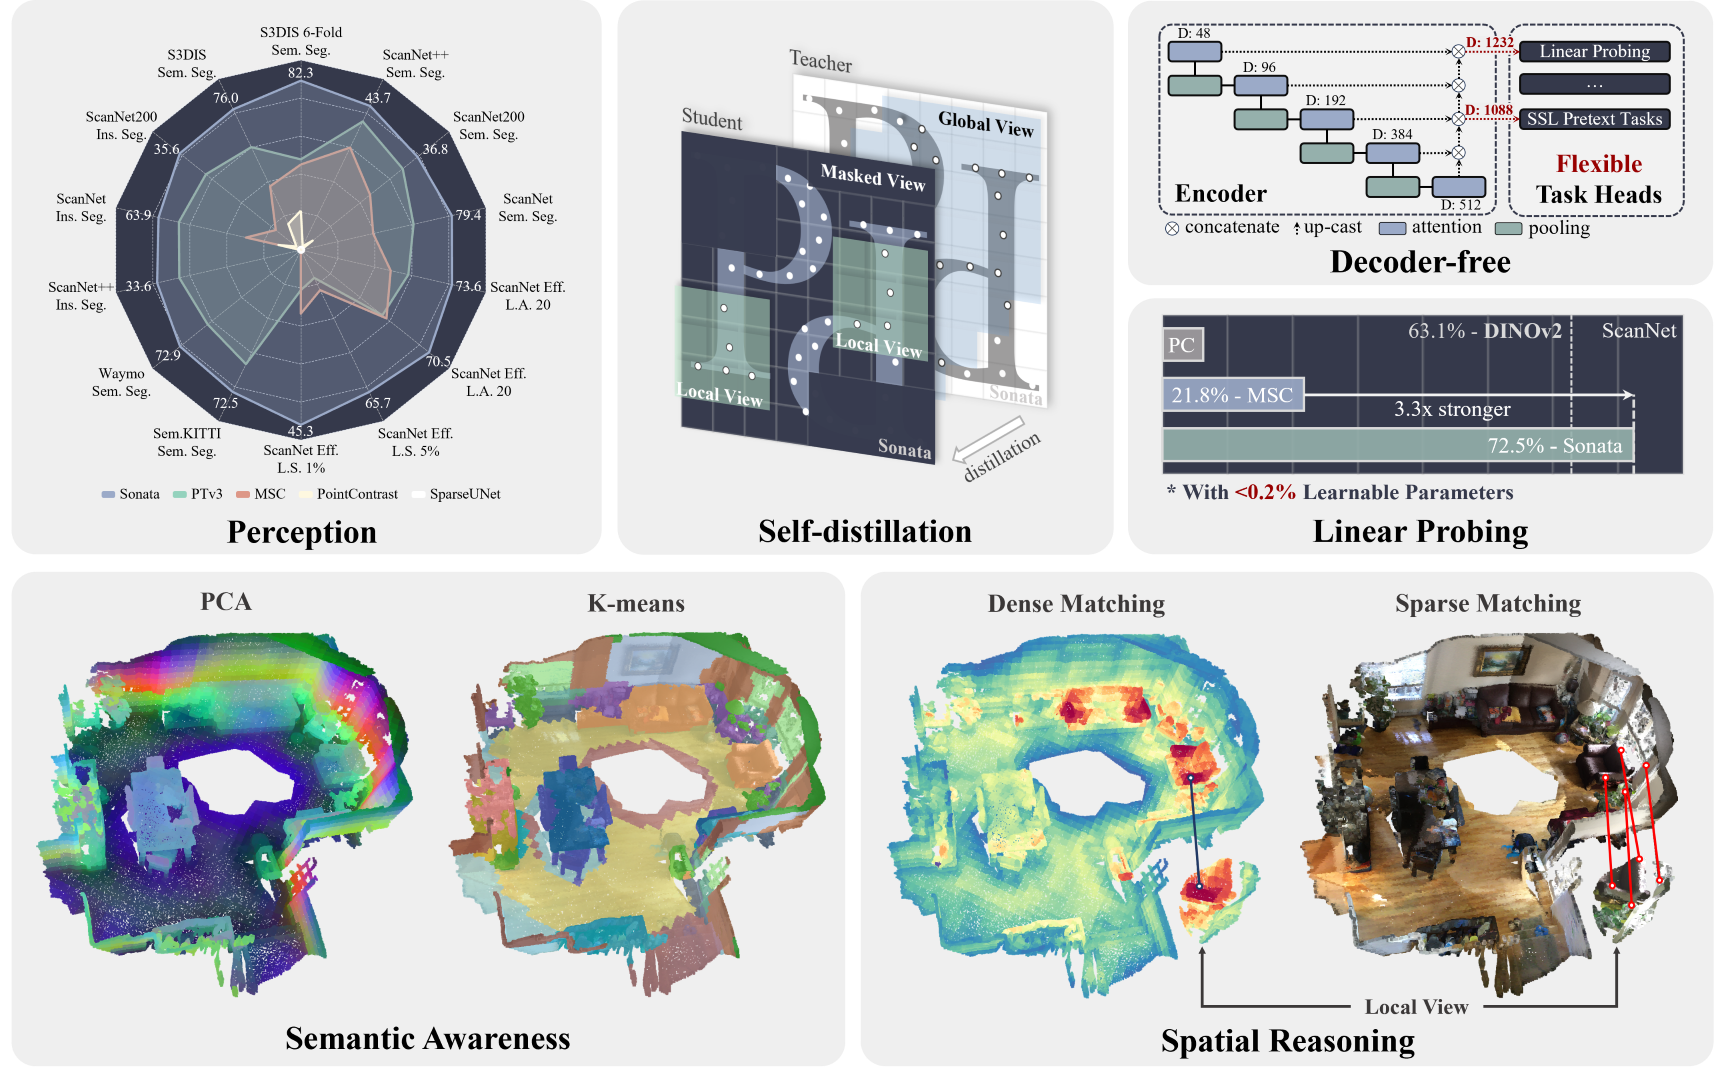
\includegraphics[width=0.7\linewidth]{figures/article-fig1-main-properties.png}
    \caption{Overview of the Sonata architecture and its emerging properties, demonstrating zero-shot semantic awareness and state-of-the-art linear probing performance.}
    \label{fig:sonata_overview}
\end{figure}

\subsection{The Geometric Shortcut Hypothesis}

The fundamental difference between 2D and 3D data lies in density and structure. In 2D images, pixels are arranged in a dense, regular grid, meaning all meaningful information is contained within the input features (colors) rather than the fixed pixel coordinates. Conversely, point clouds are inherently sparse. Because of this sparsity, 3D operators (such as sparse convolutions or point attention) must directly ingest the $(x, y, z)$ spatial coordinates to define their kernels.

\begin{figure}[htpb]
    \centering
    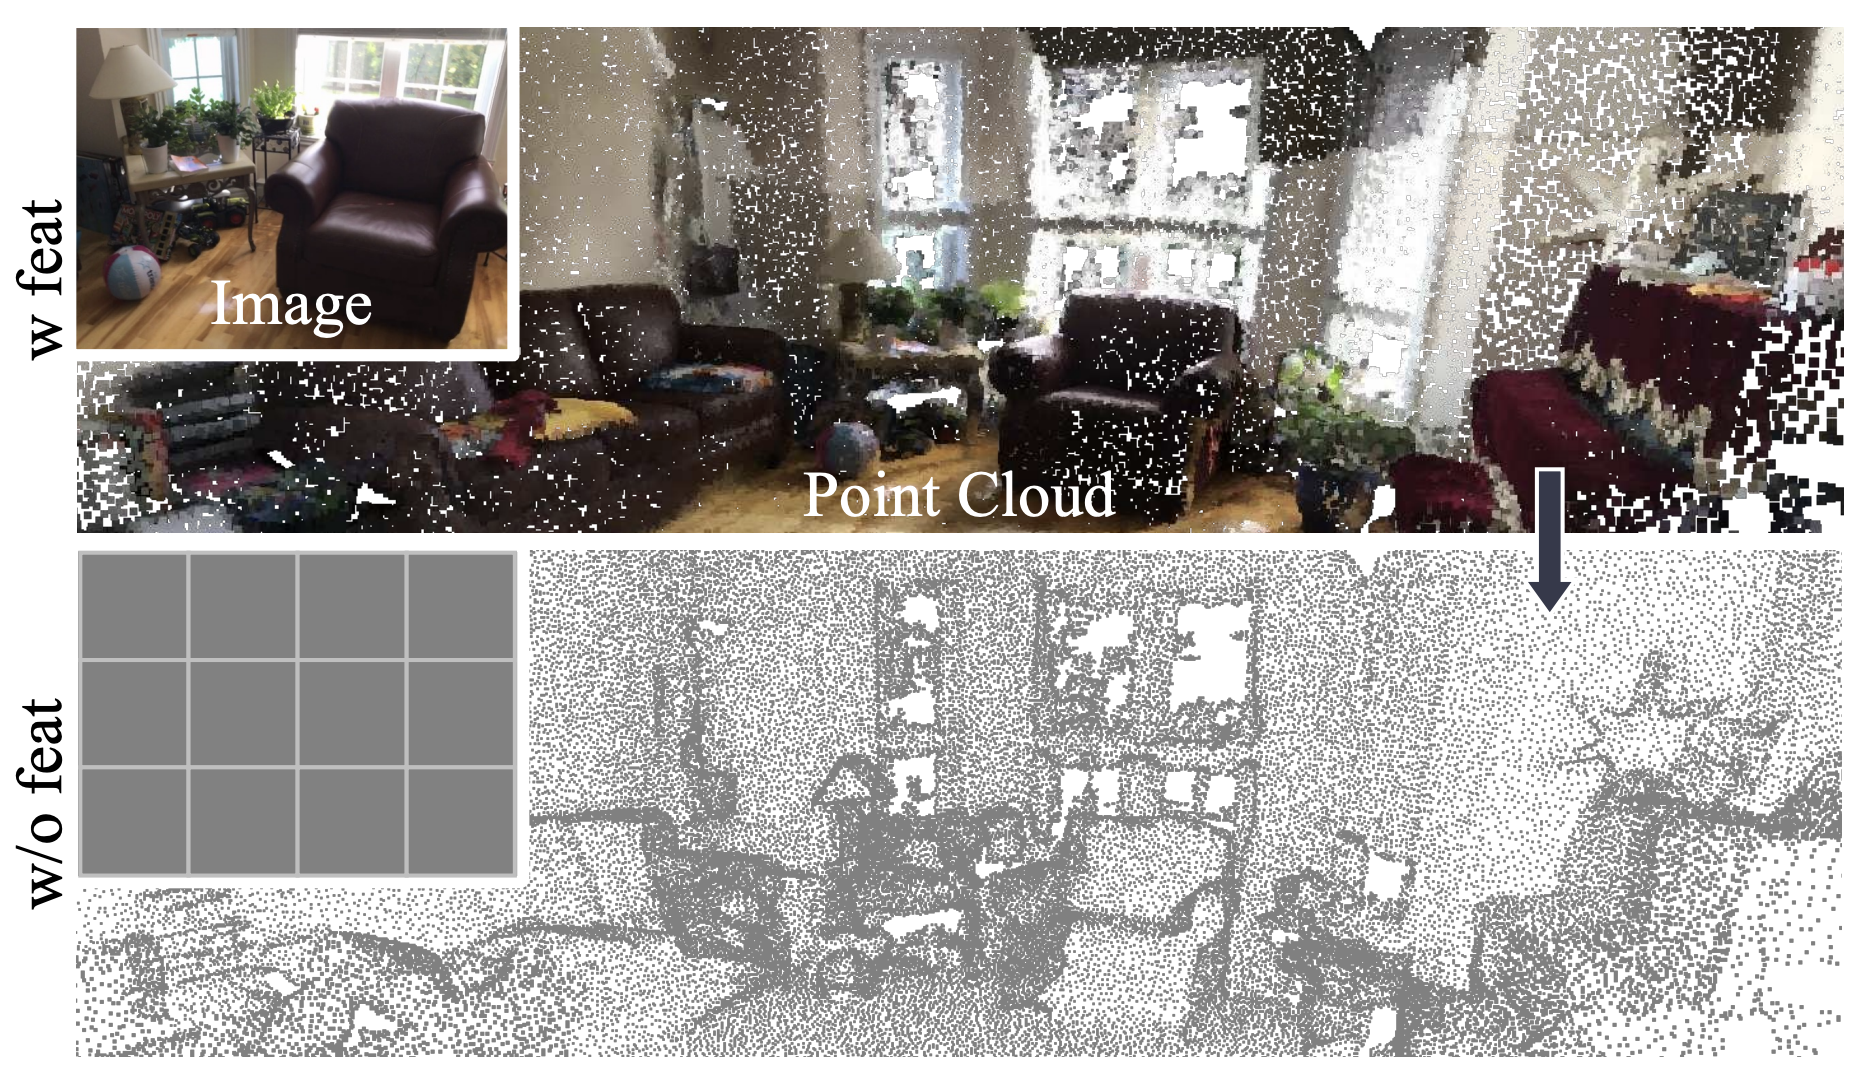
\includegraphics[width=0.7\linewidth]{figures/article-fig3-The geometric shortcut is unique to 3D.png}
    \caption{Comparison of information retention after removing input features. 3D point clouds leak structural information directly through their coordinates, unlike 2D images.}
    \label{fig:3d_vs_2d}
\end{figure}

Because spatial coordinates are perpetually fed into the network alongside the features, it becomes nearly impossible to effectively mask out spatial information during self-supervised pre-training. Consequently, when tasked with reconstructing masked regions, the network takes the path of least resistance: it relies on the absolute coordinates rather than inferring semantic context. As visualized in prior works, this results in representations that merely map local surface normals or Z-axis height. 

\begin{figure}[h]
    \centering
    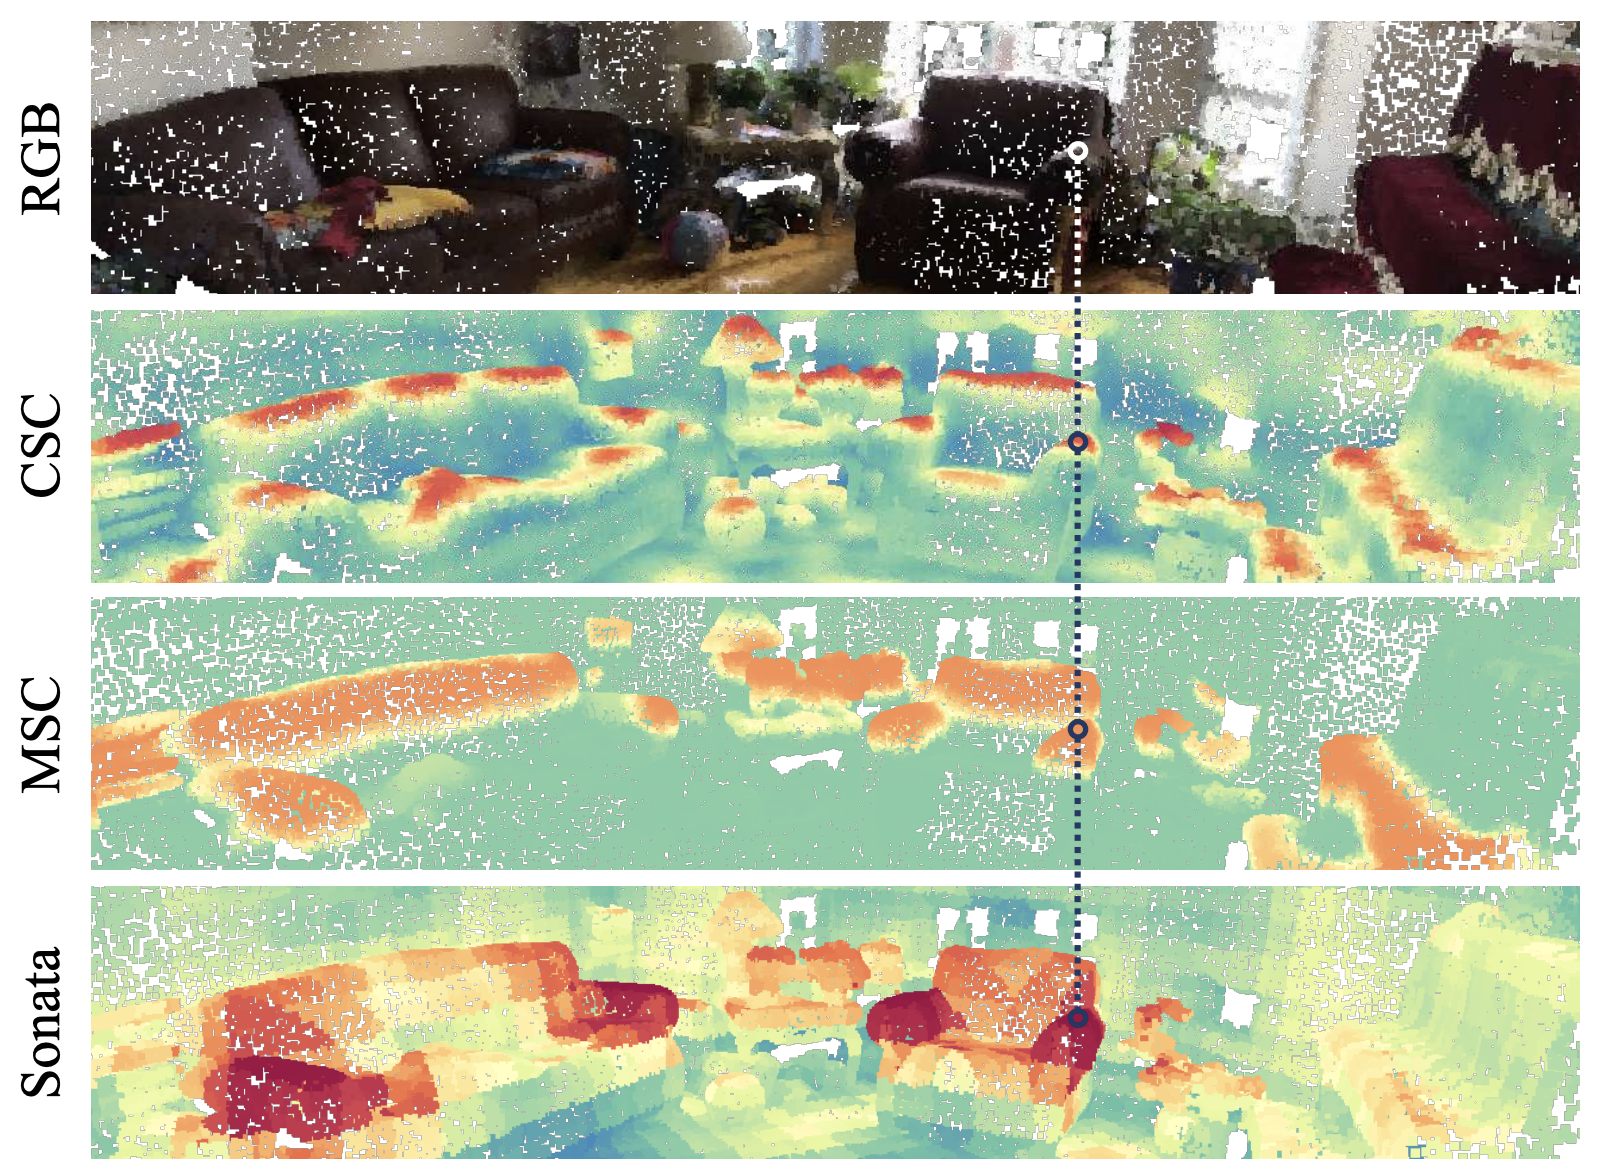
\includegraphics[width=0.7\linewidth]{figures/article-fig2-geometric-shortcut.png}
    \caption{Visualization of the geometric shortcut. Previous methods collapse to low-level geometric cues (surface normals or height), whereas Sonata groups points by semantic identity.}
    \label{fig:shortcut_heatmap}
\end{figure}

\subsection{Decoder-Free Architecture and Feature Up-casting}

Historically, 3D point cloud networks rely heavily on the U-Net architecture, utilizing a hierarchical encoder coupled with a feature-propagating decoder via skip connections. The authors of Sonata argue that decoding point clouds back to their original high-resolution scale inadvertently reintroduces fine-grained local geometric cues, facilitating the geometric shortcut. In addition, standard decoders typically restrict features to shallow channels, limiting representation capacity.

To counter this, Sonata completely removes the hierarchical decoder during pre-training. By operating strictly on the outputs of a PointTransformerV3 (PTv3) \cite{ptv3} encoder, the self-distillation loss is applied at coarser spatial resolutions, fundamentally restricting the network's access to fine-grained spatial coordinates.

However, downstream tasks like dense semantic segmentation require point-level features. To restore multi-scale context without a learned decoder, Sonata employs a parameter-free \textit{feature up-casting} process. Features are progressively up-casted back to the scale of the previous encoding stage using inverse pooling indices, and then concatenated with earlier features. This allows the model to produce dense, high-dimensional representations while bypassing the geometric pitfalls of a standard U-Net decoder.

\subsection{Additional Regularization and Self-Distillation}

Beyond architectural changes, Sonata introduces targeted masked point jittering during pre-training to further obscure spatial leakage by aggressively disrupting the spatial relationships of masked points. Moving away from traditional objectives, Sonata adapts a DINOv2-style self-distillation framework, aligning highly corrupted student views with rich, global targets from a slow-moving Exponential Moving Average teacher network.

% ==========================================
\section{Evaluation Questions and Hypotheses}
% ==========================================

While the Sonata architecture presents a compelling and highly scalable framework for 3D self-supervised learning, a rigorous theoretical inspection reveals potential vulnerabilities in its design. Before proceeding to our empirical evaluation, we outline two critical hypotheses regarding the limitations of the authors' approach.

\subsection{Hypothesis 1: Dense Up-Casting May Preserve Spatial Dependence}

The central premise of Sonata is that removing the standard U-Net decoder prevents the model from collapsing into the geometric shortcut, as the self-distillation loss is strictly applied to coarser, pooled representations \cite{sonata2025}. While this logic may hold true for the network's latent space, it introduces a critical contradiction for downstream applications. Dense perception tasks, such as point-level semantic and instance segmentation, inherently require high-resolution feature maps. 

To bridge this resolution gap, the authors employ a parameter-free feature up-casting mechanism. Coarse features are progressively mapped back to the original point density using inverse pooling indices, and then concatenated with earlier, higher-resolution feature maps. We may hypothesize that this mechanism may preserve or reintroduce dependence on absolute spatial structure. The later experiments are designed to test whether the final dense features remain strongly predictive of coordinates. 

If this hypothesis is supported, it would suggest that the construction of dense point-level features may preserve or reintroduce substantial low-level spatial information. Confirming this interpretation would require direct comparison with coarse pre-up-casting features.

\subsection{Hypothesis 2: The Geometric Ceiling in Visually Ambiguous Regions}

This second hypothesis is not directly tested in the present report; rather, it serves as a broader interpretive lens for discussing the limits of purely geometric self-supervised learning. Beyond architectural mechanisms, purely 3D self-supervised models face an inherent data modality limitation, which we term the ``geometric ceiling.'' The Sonata pretext tasks rely heavily on spatial structural perturbations and masked point predictions to induce object semantics. However, in standard indoor environments, semantics are often decoupled from structural geometry. 

To illustrate this , let's consider a flat wall on which lies a whiteboard, a poster, and a TV. Geometrically, these objects are nearly indistinguishable as they are all planar surfaces with small structural variance. A purely 3D model like Sonata lacks the visual details needed to distinguish between them, inevitably clustering them into a single semantic group. 

While the authors demonstrate that Sonata achieves state-of-the-art linear probing, we argue that pure 3D SSL cannot reach the semantic granularity of 2D visual foundation models (such as DINOv2 \cite{dinov2}) without explicit multimodal fusion. The inability to resolve photometric ambiguity using point coordinates and sparse colors alone remains a hard upper bound on the model's zero-shot semantic capabilities.

% ==========================================
\section{Experimental Methodology}
% [~1.5 pages]
% Explain the setup of your code contribution on the MesoNET (Juliet) cluster.


Before analyzing the features extracted by the pre-trained Sonata backbone on real-world datasets, it is imperative to rigorously validate our proposed evaluation metrics. We must empirically validate that our diagnostic tools can distinguish between strongly geometry-dominated representations and more semantically structured ones. To achieve this, we designed a synthetic control experiment (Sanity Check) on the Juliet cluster.

\subsection{Experimental Design: The Synthetic Sanity Check}
We generated a synthetic 3D point cloud comprising $N=12000$ points, uniformly distributed such that coordinates $(x, y, z) \in [-1, 1]^3$. For this point cloud, we constructed two contrasting high-dimensional feature representations ($D=32$):

\begin{enumerate}
    \item \textbf{Shortcut Baseline ($\phi_{shortcut}$):} This matrix simulates a neural network that has suffered severe geometric collapse. We construct it by explicitly concatenating and tiling the raw $(x, y, z)$ spatial coordinates to fill the 32 dimensions. These tiled coordinates are assigned a dominant weight, while a minor semantic noise vector is added to prevent mathematical singularity. The resulting representation is overwhelmingly dominated by absolute spatial location, acting as a worst-case baseline.
    \item \textbf{Semantic Like ($\phi_{semantic}$):} This matrix simulates a more semantically structured representation, intended to encode class-level structure while retaining weak geometric traces, echoing the objectives of the Sonata architecture. First, we partition the point cloud into four distinct, non-axis-aligned "semantic classes" using non-linear spatial thresholds (radial distance and polar angles). Each class is assigned an ideal 32-dimensional semantic centroid. The feature vector for each point is heavily weighted towards its corresponding centroid. However, because no real-world network is perfectly free of geometric leakage, we inject a faint trace of the raw spatial coordinates as background noise. 
\end{enumerate}

\begin{figure}[h]
\centering
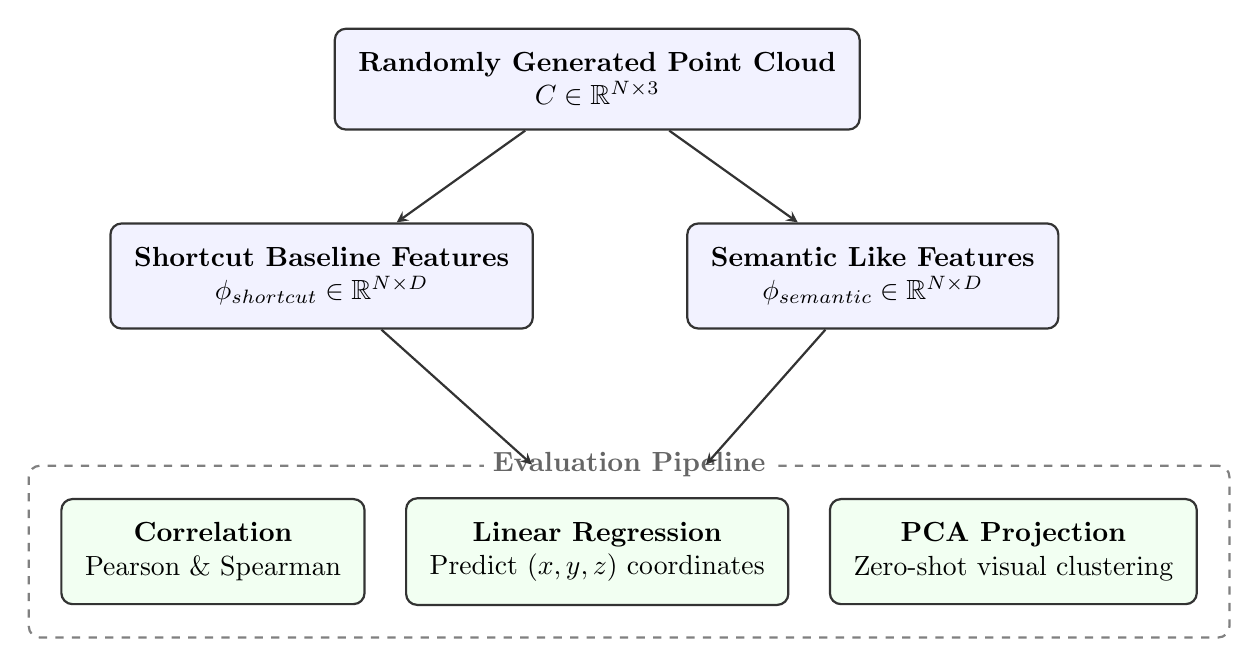
\begin{tikzpicture}[
    % Define simple, standard styles
    box/.style={rectangle, draw=black!80, thick, align=center, rounded corners, minimum height=1cm, inner sep=0.3cm, fill=blue!5},
    evalbox/.style={rectangle, draw=black!80, thick, align=center, rounded corners, minimum height=1cm, inner sep=0.3cm, fill=green!5},
    arrow/.style={thick, ->, >=stealth, draw=black!80}
]

% 1. Top Node: The Point Cloud
\node[box] (pc) at (0, 0) {\textbf{Randomly Generated Point Cloud} \\ $C \in \mathbb{R}^{N \times 3}$};

% 2. Middle Nodes: The Two Feature Types
\node[box] (shortcut) at (-3.5, -2.5) {\textbf{Shortcut Baseline Features} \\ $\phi_{shortcut} \in \mathbb{R}^{N \times D}$};
\node[box] (semantic) at (3.5, -2.5) {\textbf{Semantic Like Features} \\ $\phi_{semantic} \in \mathbb{R}^{N \times D}$};

% 3. Evaluation Block (Grouped)
\node[evalbox] (linreg) at (0, -6) {\textbf{Linear Regression} \\ Predict $(x, y, z)$ coordinates};
\node[evalbox, left=0.5cm of linreg] (corr) {\textbf{Correlation} \\ Pearson \& Spearman};
\node[evalbox, right=0.5cm of linreg] (pca) {\textbf{PCA Projection} \\ Zero-shot visual clustering};

% Draw a dashed box around the evaluation metrics
\node[draw=gray, dashed, thick, rounded corners, inner sep=0.4cm, fit=(linreg) (corr) (pca)] (evalbox) {};
\node[fill=white, text=gray!80!black, font=\bfseries] at (evalbox.north) {Evaluation Pipeline};

% Draw the connecting arrows
\draw[arrow] (pc) -- (shortcut);
\draw[arrow] (pc) -- (semantic);
\draw[arrow] (shortcut) -- (evalbox);
\draw[arrow] (semantic) -- (evalbox);

\end{tikzpicture}
\caption{Workflow of the synthetic control experiment. A random point cloud is used to generate two contrasting feature spaces, which are then evaluated on how easily their absolute coordinates can be extracted via linear regression.}
\label{fig:synthetic_workflow_simple}
\end{figure}

\subsection{Evaluation Methodology}
To quantify the degree of geometric leakage in these representations, we employ two primary metrics:

\paragraph{1. Coordinate Predictability via Linear Probing ($R^2$):} 
If a representation relies heavily on geometric shortcuts, a simple linear transformation should be able to recover the absolute coordinates from the feature vectors. To measure this, we fit a linear regressor (via least squares) mapping the $D$-dimensional features to the 3D coordinates using 70\% of the points as a training set. The predictive power is evaluated on the remaining 30\% using the coefficient of determination, $R^2$. Let $y_i$ denote the ground-truth spatial coordinate (e.g., $x$, $y$, or $z$) for the $i$-th point in the test set, $\hat{y}_i$ be the corresponding coordinate predicted by our linear model, and $\bar{y}$ be the mean of the ground-truth coordinates across the test set. The metric is computed as:
$$ R^2 = 1 - \frac{\sum_{i} (y_i - \hat{y}_i)^2}{\sum_{i} (y_i - \bar{y})^2} $$
An $R^2$ score approaching 1.0 indicates severe geometric collapse, meaning the feature space collectively memorizes physical space.

\paragraph{2. Feature-Geometry Correlation:}
While $R^2$ evaluates the feature space collectively, correlation metrics detect if any single feature dimension explicitly memorizes a spatial axis. To formulate this, let $N$ be the total number of points in the point cloud. We define $F_d$ as the activation values of a specific feature dimension $d$ across all points, where $F_{d,i}$ is the value for the $i$-th point and $\bar{F}_d$ is its mean activation. Similarly, let $C_a$ represent a specific spatial coordinate axis, with $C_{a,i}$ being the coordinate of the $i$-th point and $\bar{C}_a$ being the axis mean. We compute the maximum absolute values of two distinct correlation metrics:

\begin{itemize}
    \item \textbf{Pearson Correlation Coefficient ($|r|$)} measures strict linear dependence, identifying if a specific neuron acts as a direct, scaled proxy for an absolute coordinate. It is computed as the covariance of the feature and coordinate divided by the product of their standard deviations:
    $$ r = \frac{\sum_{i=1}^{N} (F_{d,i} - \bar{F}_d)(C_{a,i} - \bar{C}_a)}{\sqrt{\sum_{i=1}^{N} (F_{d,i} - \bar{F}_d)^2 \sum_{i=1}^{N} (C_{a,i} - \bar{C}_a)^2}} $$
    
    \item \textbf{Spearman Rank Correlation Coefficient ($|\rho|$)} assesses monotonic dependence. It captures non-linear geometric leakage introduced by network activation functions (e.g., ReLU or GELU) and detects features that strictly increase or decrease along a spatial axis, even if the relationship lacks perfect linearity. It is computed based on $d_i$, which is the difference between the ordinal rank of the feature value, $\text{rank}(F_{d,i})$, and the ordinal rank of the spatial coordinate, $\text{rank}(C_{a,i})$, for the $i$-th point:
    $$ \rho = 1 - \frac{6 \sum_{i=1}^{N} d_i^2}{N(N^2 - 1)} $$
\end{itemize}

By extracting the maximum absolute values of these correlation metrics across all $D$ feature dimensions, we establish a worst-case boundary. If the network successfully disentangles semantics from geometry, no single feature should act as a proxy for physical space, resulting in uniformly low maximum correlation scores.

\subsection{Quantitative Results}
The evaluation script successfully distinguished between the two synthetic representations, passing the automated sanity check. The metrics are summarized in Table \ref{tab:synthetic_metrics}.

\begin{table}[h]
    \centering
    \begin{tabular}{@{}lcc@{}}
        \toprule
        \textbf{Metric} & \textbf{Shortcut Baseline} & \textbf{Semantic Like} \\ \midrule
        Mean Linear Probe $R^2$ & \textbf{0.9997} & 0.6502 \\
        \hspace{3mm} $x$-axis $R^2$ & 0.9998 & 0.6273 \\
        \hspace{3mm} $y$-axis $R^2$ & 0.9997 & 0.6832 \\
        \hspace{3mm} $z$-axis $R^2$ & 0.9997 & 0.6401 \\ \midrule
        Mean Pearson $|r|$ & \textbf{0.9444} & 0.1963 \\
        Mean Spearman $|\rho|$ & \textbf{0.9475} & 0.2205 \\ \bottomrule
    \end{tabular}
    
    \caption{Geometric Leakage Metrics on Synthetic Representations ($N=12000$, $D=32$)}
    \label{tab:synthetic_metrics}
\end{table}

The \textit{Shortcut Baseline} yielded an $R^2$ of nearly 1.0 across all axes, indicating that the metric correctly identifies explicitly spatial patterns. In contrast, the \textit{Semantic Like} features restricted the linear probe to an average $R^2$ of 0.6502, while the mean Pearson correlation plummeted from 0.9444 to 0.1963. This substantial numerical gap suggests the sensitivity of our metric to strong geometric encoding. Structured representations can still retain some coordinate information. The metric should therefore be interpreted as capturing the degree of geometric predictability rather than establishing an absolute presence or absence of a shortcut.

\subsection{Qualitative Visualization (Zero-Shot PCA)}
To visually corroborate the statistical findings, we computed a 2D Principal Component Analysis (PCA) projection of both feature spaces. 

\begin{figure}[h]
    
    \centering
    
    \begin{minipage}{0.48\textwidth}
        \centering
        \boxed{
        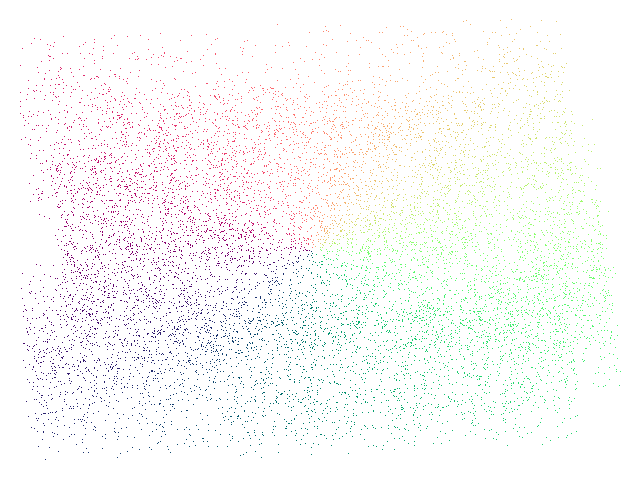
\includegraphics[width=\linewidth]{figures/shortcut_baseline_pca.png}
        }
        \caption{PCA projection of the \textit{Shortcut Baseline}. The rigid, uniform structure reflects pure geometric memorization.}
        \label{fig:pca_shortcut}
    \end{minipage}\hfill
    \begin{minipage}{0.48\textwidth}
        \centering
        \boxed{
        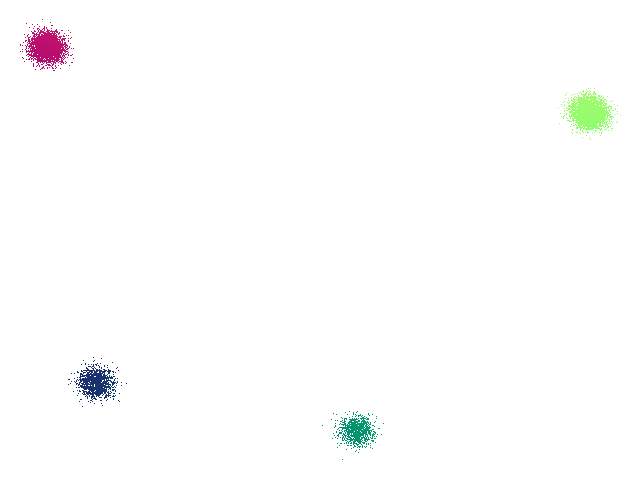
\includegraphics[width=\linewidth]{figures/semantic_like_pca.png}
        }
        \caption{PCA projection of the \textit{Semantic Like} features. Distinct clustering reflects learned semantic groupings.}
        \label{fig:pca_semantic}
    \end{minipage}
\end{figure}

As shown in Figure \ref{fig:pca_shortcut}, the PCA of the shortcut representation forms a homogeneous continuous shape. Because the "features" are largely spatial coordinates, the projection simply unwraps the physical geometry of the point cloud. Conversely, Figure \ref{fig:pca_semantic} demonstrates that semantic-driven features naturally break apart into distinct functional clusters, thoroughly disrupting the continuous spatial mapping.

\subsection{Conclusion of the Sanity Check}
The successful execution of this synthetic experiment verifies our diagnostic pipeline. We have shown empirically, both quantitatively and visually, that our metrics are sensitive to strong geometric encoding. With the analytical framework validated, we can now proceed to Axis 1 of our study: extracting real features using the pre-trained Sonata model on ScanNet point clouds and feeding them into this exact evaluation pipeline.


\subsection{Implementation Details}

All experiments were conducted on the MesoNET (Juliet) computing cluster. Feature extraction was performed using a single NVIDIA A100 GPU (80GB) to accommodate the 108M parameter PointTransformerV3 (PTv3) Sonata backbone. The evaluation pipeline, including the linear regression probes and PCA projections, was executed on CPU nodes. The software environment utilized PyTorch 2.5.0 with CUDA 12.4.

For all probing experiments, we randomly split points from the single indoor scene into 70\% training and 30\% test subsets. We fit one independent least-squares linear regressor per coordinate axis. Features were used in their raw extracted form ($D=1088$) without additional L2-normalization, and target coordinates were standardized (centered and scaled) before regression. Results reported in the tables correspond to a single random split, which was verified across several random seeds to ensure stability.

The complete source code for feature extraction, linear probing, and PCA visualization is open-source and available at: \url{https://github.com/rubenifrah/SONATA-project}.

% ==========================================
\section{Results and Empirical Analysis}
% ==========================================

With our evaluation metric validated, we proceed to extract and analyze the dense representations produced by the pre-trained Sonata backbone on indoor scenes. 

We conduct a focused case study on one unseen indoor point cloud to test whether Sonata's final dense features remain strongly predictive of absolute coordinates in practice. For this case study, suitable raw indoor \texttt{.ply} scans were limited, so we used an unseen indoor scan, \texttt{indoor\_scan.ply}, from the first practical session of the course. The scan was downsampled to $N=273,530$ points to match the density of standard ScanNet fragments, and dense features were extracted using the official 108M-parameter Sonata model on an A100 GPU.

\subsection{Quantifying the Geometric Shortcut in Sonata}

The core claim of the Sonata architecture is that by removing the standard U-Net decoder and applying self-distillation on coarser scales, the network is forced to learn robust semantics rather than collapsing into the ``geometric shortcut''. 

To rigorously test this claim, we intercepted Sonata's dense representations ($D=1088$) after the parameter-free feature up-casting phase. We then evaluated whether the final dense representations retain strong linear predictability of absolute coordinates $(x, y, z)$ using our previously validated probe.

The quantitative results of this probe are summarized in Table \ref{tab:sonata_r2_results}, alongside synthetic control representations used only to illustrate the behavior of the probing metric.

\begin{table}[htpb]
    \centering
    \begin{tabular}{@{}lccc@{}}
        \toprule
        \textbf{Metric} & \textbf{Synthetic Shortcut} & \textbf{Synthetic Semantic} & \textbf{Sonata (Dense Features)} \\ \midrule
        \textbf{Mean Probe $R^2$} & \textbf{0.999} & \textbf{0.650} & \textbf{0.988} \\
        \hspace{3mm} $x$-axis $R^2$ & 0.999 & 0.627 & 0.981 \\
        \hspace{3mm} $y$-axis $R^2$ & 0.999 & 0.683 & 0.985 \\
        \hspace{3mm} $z$-axis $R^2$ & 0.999 & 0.640 & 0.997 \\ \midrule
        \textbf{Mean Pearson $|r|$} & 0.944 & 0.196 & 0.219 \\
        \textbf{Mean Spearman $|\rho|$} & 0.947 & 0.220 & 0.223 \\ \bottomrule
    \end{tabular}
    
    \caption{Linear Probing for Geometric Leakage. Sonata's dense up-casted features are shown together with synthetic control representations that illustrate highly geometry-dominated and more semantically structured feature spaces.}
    \label{tab:sonata_r2_results}
\end{table}

\subsubsection*{Distributed vs. Explicit Geometric Leakage}

An important mathematical nuance emerges when comparing the linear probe to the correlation metrics. While the linear probe $R^2$ score is nearly perfect ($0.988$), the maximum absolute Pearson correlation remains relatively low ($0.219$). This discrepancy reveals the nature of Sonata's geometric leakage: it is highly distributed. 

Unlike our synthetic baseline, which explicitly copied spatial coordinates into single feature dimensions (yielding a Pearson correlation of $0.94$), Sonata distributes spatial data across the 1088-dimensional latent space. No single neuron acts as a direct "GPS coordinate", which successfully fools basic correlation checks. However, the linear combination of the ensemble perfectly reconstructs physical space, indicating that strong spatial dependence has merely been obfuscated, not eliminated.

\subsection{Critical Analysis of the Feature Up-Casting Mechanism}

The empirical results raise an important tension with the architectural intuition presented in the original paper.

This mathematical conclusion is strikingly corroborated by visual evidence. As shown in Figure \ref{fig:indoor_scan_pca}, when Sonata's dense features are projected into RGB space via a 6-component PCA blend (replicating the authors' exact visualization methodology), the resulting point cloud does not exhibit discrete semantic clusters. 

\begin{figure}[H]
    \centering
    \begin{subfigure}{0.48\textwidth}
        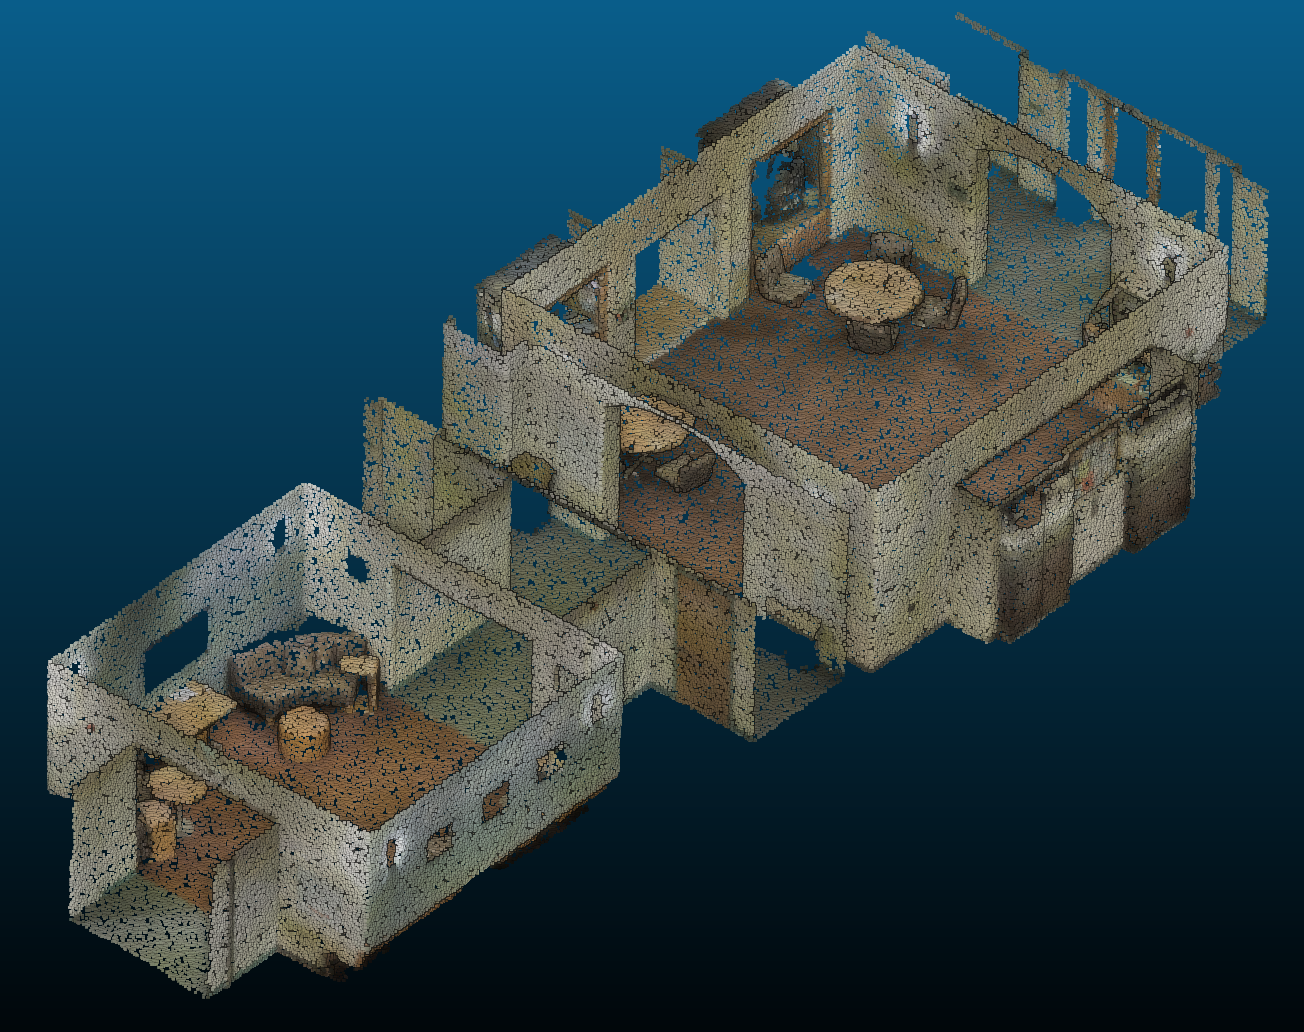
\includegraphics[width=\linewidth]{figures/cc_indoor_scan.png}
        \caption{Original Scan}
    \end{subfigure}\hfill
    \begin{subfigure}{0.48\textwidth}
        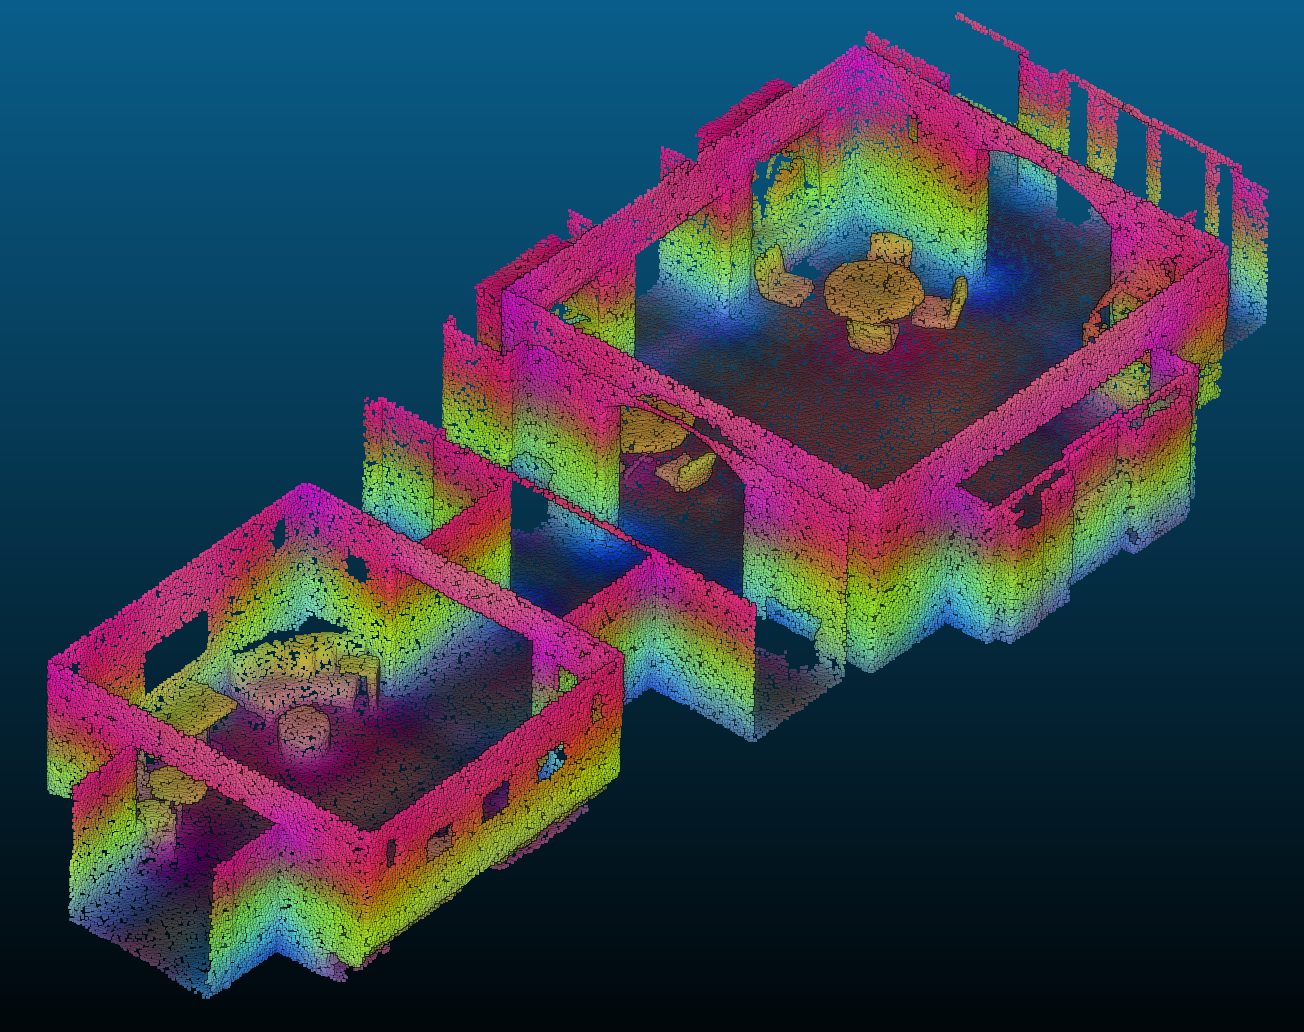
\includegraphics[width=\linewidth]{figures/cc_indoor_scan_pca.png}
        \caption{Zero-Shot PCA of Dense Features}
    \end{subfigure}
    \caption{Comparison of the original indoor point cloud (left) and the 6-component PCA projection of Sonata's dense up-casted features (right). Rather than grouping objects by semantic identity, the PCA colors form continuous spatial gradients across the room, visually confirming the geometric leakage quantified by the linear probe.}
    \label{fig:indoor_scan_pca}
\end{figure}


Instead of grouping structurally similar objects (e.g., all tables or all chairs) under a uniform color, the feature space forms a continuous, unbroken gradient across the physical geometry of the room. The colors transition smoothly from one end of a wall to the other, and from the floor up to the ceiling. This gradient is visually consistent with a representation dominated by geometric encoding, mirroring the behavior of the strongly geometry-dominated baseline we synthesized in our earlier control experiment.

We hypothesize that this leakage may be a consequence of the parameter-free feature up-casting mechanism. While Sonata successfully removes the parametric U-Net decoder to prevent spatial leakage during pre-training, the necessity to perform dense prediction tasks (like semantic segmentation) requires projecting coarse features back to the original high-resolution points. Because this up-casting relies on concatenating features using inverse pooling indices, which are strictly defined by local geometric proximity, it arguably preserves or reintroduces spatial dependence in the final dense representation. 

This finding suggests a potential architectural limitation: while the latent coarse features may be more semantic, the construction of dense point-level features may preserve or reintroduce substantial low-level spatial information. At this stage, our experiments do not isolate causality: they show that the final dense representations remain strongly geometry-predictive, but they do not yet prove that feature up-casting is the unique source of this effect. Confirming this interpretation would require direct comparison with coarse pre-up-casting features.

\newpage
% ==========================================
% ==========================================
\section{Discussion and Future Work}
% ==========================================

Our empirical findings present an important caveat to the claims made by the Sonata authors \cite{sonata2025}. While the self-distillation framework and decoder-free architecture may foster strong semantic learning in the latent space, the construction of dense point-level features may preserve or reintroduce substantial low-level spatial information. The resulting representation appears highly structured by spatial coordinates in this case study, as evidenced by our $R^2 = 0.988$ probe and the continuous PCA color gradients.

Given these findings, we propose two critical directions for future work to fully evaluate and potentially rectify the Sonata architecture:

\paragraph{1. Architectural Ablation: Coarse vs. Dense Features}
To isolate the exact source of the geometric collapse, future experiments must ablate the feature extraction pipeline. By applying our linear regression probe directly to the coarse, grid-sampled features extracted immediately after the PTv3 \cite{ptv3} encoder (prior to any inverse pooling or up-casting) we could determine if the encoder itself successfully suppresses the geometric shortcut. If the coarse features yield a substantially lower $R^2$ score than the dense features, this would strongly support the hypothesis that dense feature construction (rather than the coarse encoder alone) plays a major role in the observed spatial predictability.

\paragraph{2. The Geometric Ceiling and Multimodal Fusion}
Beyond the findings directly supported by our experiments, a broader limitation of purely geometric 3D SSL concerns an inherent "geometric ceiling." In environments with rich visual semantics but flat geometry (e.g., posters on a wall, whiteboards, or screens), point coordinates and structural features are insufficient to distinguish object classes, as mentioned previously. Future work should investigate cross-modal distillation, leveraging 2D foundation models like DINOv2 \cite{dinov2}. By fusing pixel-aligned DINOv2 photometric features with Sonata's structural features, the model could bridge the gap between pure geometric reasoning and fine-grained visual semantics, yielding a truly robust representation.

\paragraph{Limitations}
This study has several limitations. First, the real-scene analysis is currently conducted on a single indoor scan, so the conclusions should be interpreted as a focused case study rather than a definitive benchmark. Indeed, it was actually very difficult for us to find ready-to-use open-sourced indoor scans of good quality. We thus decided to rely on the known \texttt{indoor\_scan} already used several times throughout the course's TPs. Second, we analyze only the final dense features and not the intermediate coarse features, so the precise architectural source of the observed spatial predictability remains unresolved. Third, strong coordinate predictability does not imply the absence of semantic content: it only shows that substantial geometric information remains linearly recoverable from the representation.

\section{Conclusion}
In this report, we evaluated key aspects of the Sonata 3D SSL framework. After validating our proposed linear probe on synthetic controls, we applied it to an unseen indoor scan and found that Sonata's dense representations remain highly predictive of absolute spatial coordinates in this case study. We do not claim to have refuted Sonata at all, however, these findings raise important cautions about the interpretation of dense 3D SSL features. The precise source of this predictability remains to be isolated, motivating a more careful examination of how dense point-level features are constructed and evaluated. More broadly, this report illustrates how simple probing tools can provide useful diagnostics for evaluating whether dense 3D self-supervised representations remain overly tied to raw geometry.

% --- References ---
\bibliographystyle{plain}
\begin{thebibliography}{9}

\bibitem{sonata2025}
Z. Runyan et al.,
\textit{Sonata: Self-Supervised Learning of Reliable Point Representations},
CVPR, 2025.

\bibitem{ptv3}
X. Xiaoyang et al.,
\textit{PointTransformerV3: Simpler, Faster, Stronger},
CVPR, 2024.

\bibitem{dinov2}
M. Oquab et al.,
\textit{DINOv2: Learning Robust Visual Features without Supervision},
TMLR, 2023.

\end{thebibliography}

\end{document}


